The groundlaying principles of the Smartsoft Architecture will be pointed out in the following
Sections. A generall overview of how components work together with the sequencer and the instruction planner will be discussed.
Aswell as the placment of the code (which machine runs which part of the software and also how are they connected).

\section{SmartSoft}
Smartsoft is designed as a Development Framework for Robots to operate in multiple Situations.
Therefor it consists multiple abstraction Layers that base on the principle of
locality. \\
The general Idea is that a Robot should be able to handle as much work as it is locally enabled to do.
Just when an Error occurs that the Robot is unable to fix by itself it will escalate the Problem to the next higher instance. \\
\\
\begin{figure}[h]
\centering
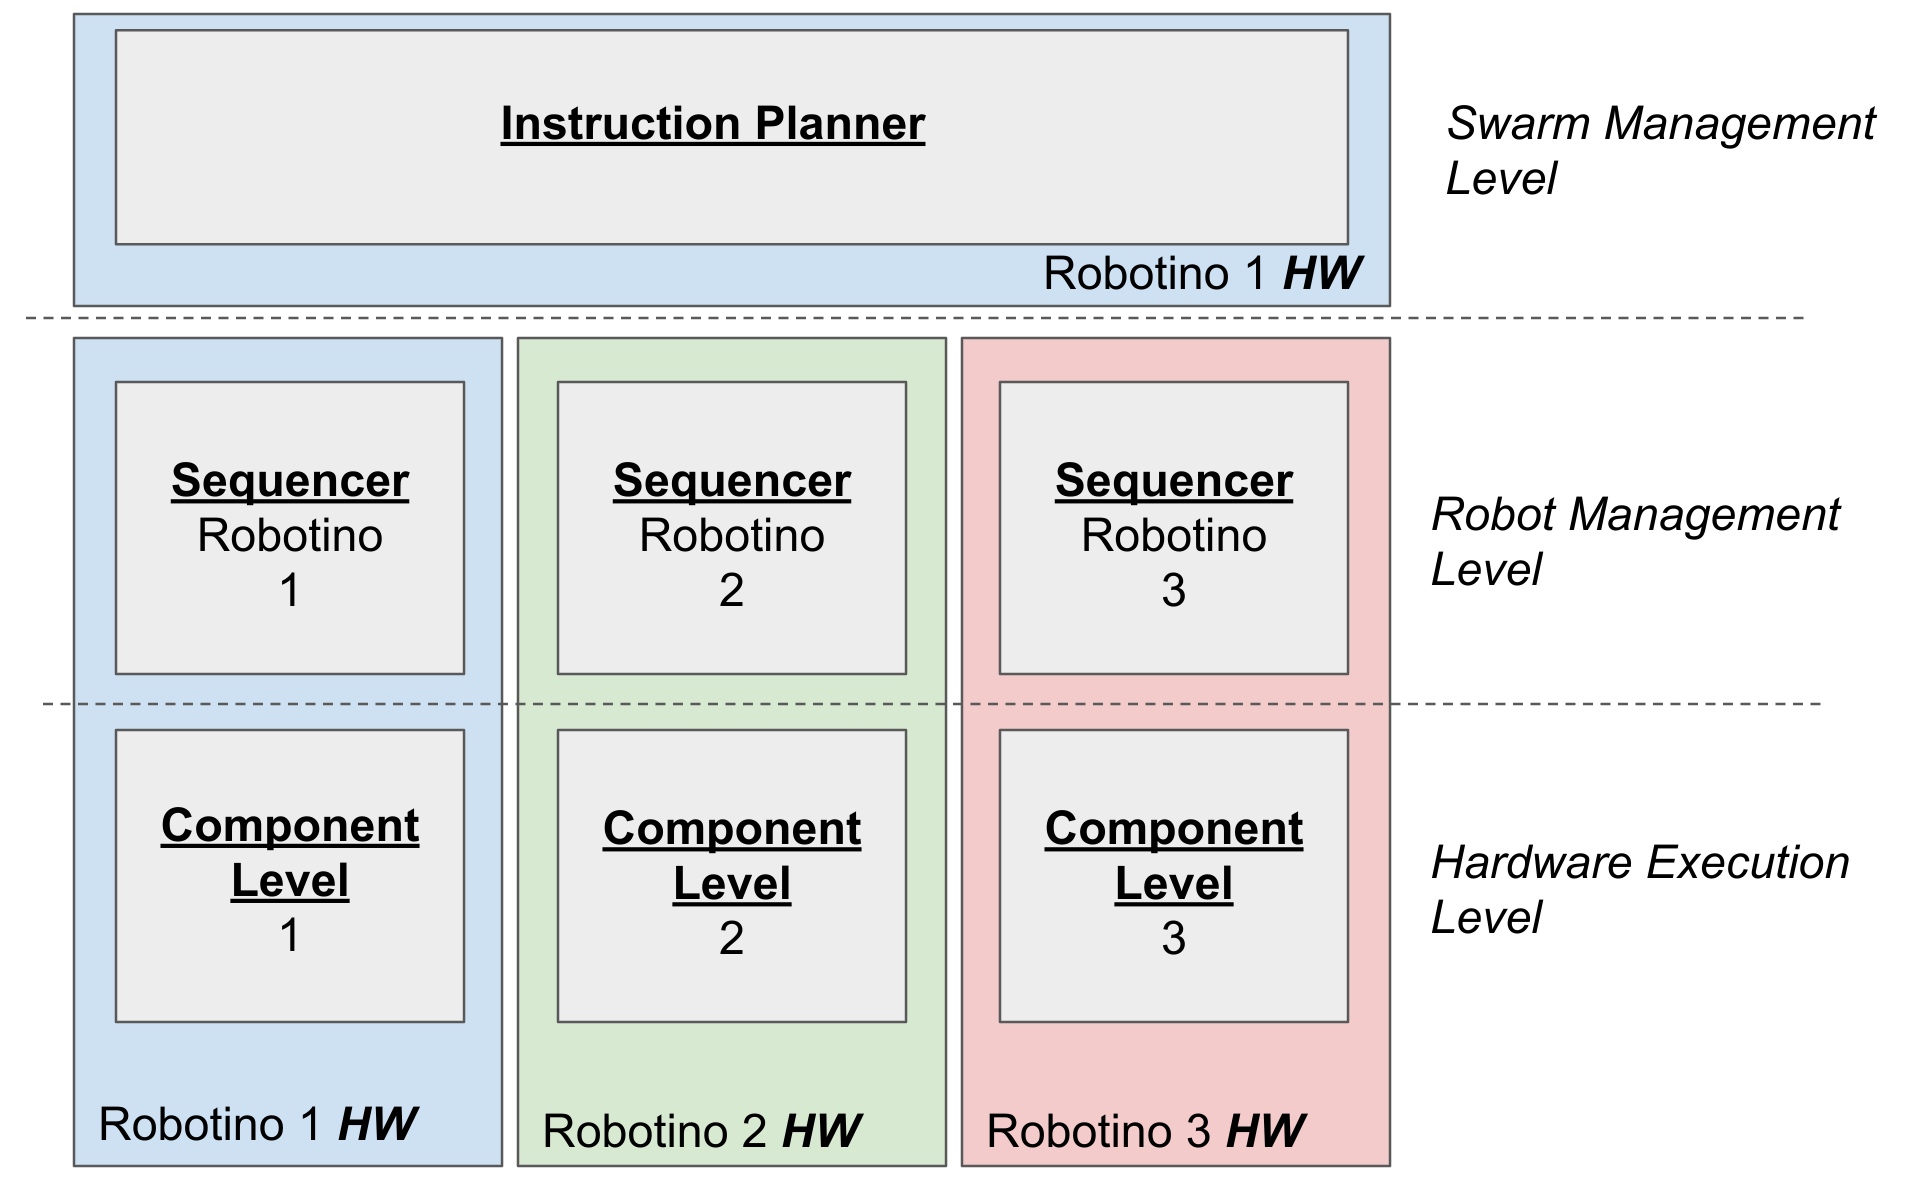
\includegraphics[scale=0.23]{pic/architecture2018.png}
\caption{Arrangement of Components in Architecture}
\label{fig:architecture_overview}
\end{figure}

This leads to a distributed system with several parts of the software running on different machines, our robots.
As seen in the picture above \ref{fig:architecture_overview}, some parts of the system run as a copy on every robot
(e.g. the sequencer or movement dependent components). we will take a closer look at these parts later in this document. \\
\\

\subsection{Instruction Planner}
The instruction planner will take care that the Task it has been assigned to the system will be handled
in a effective way. It consists of multiple parts, the \textbf{Fleet Management} and the \textbf{Objective Management} (see \ref{ch:SmartRobotinoInstructionPlanner}). \\
\\
It actually does not matter on which machine the instruction planner is deployed, it could be an external computer,
or just like in our case, one of the Robotinos that are deployed on the field.\\
The limitation is that the instruction planner has to:
\begin{itemize}
    \item have a stable connection to all other robots
    \item as well as the refbox
    \item be unique
\end{itemize}
Especially the uniqueness is one point that has to be considered in further progress of the System.
This problem might lead to problems with future deployments of multiple robot systems (see \ref{subsec:Deployments}). \\
\\
The purpose of the instruction planner is to keep track of both the game and the robots that are participating.
Based on the information that is provided by all the robots, the instruction planner will decide which
robot has to perform which task.

\subsection{Sequencer}
(also the Sequencer is often referred to as the \textit{"LispServer"})
The Sequencer manages events that occur locally at the robotino it has been deployed on.
Its purpose is to manage all situations that are not "mission critically" and can be solved by the robotino itself. \\
A good example is the collision free movement:
The robotinos are able to apprach a position on the field without hitting objects in their way. This needs the coordination of
multiple components inside of the robotino, e.g. the \textit{Laser scanner} and the \textit{Moving components}.
These components work together in a way that the receives events from both to process and delegate further instructions,
to avoid the crash into objects.\\
\\
The purpose of the Sequencer is to maintain control of all situations that a single robot can handle on its own.
Based on the information which other components send as events.

\subsection{Components}
Components are the most low level implementations of tasks, they handle just one special task.
E.g. they handle the movement of the Robotinos wheels, so there is one component that actually
works with the electrical Motors inside the Robotino to move the wheels.
Also all other mentioned Parts, as the Sequencer or the instruction planner are also components
that can be deployed. In these cases the components do not provide senser data, but the prepared data
e.g. from multiple sensors. They also receive and generate events. \\
\\
All these components communicate with each other using events that are delegated by the Sequencer.
The purpose of the components is the interface to the hardware or software that they handle.
Based on actual sensor values and information delegated by the Sequencer, components fulfill only very fine granular tasks.

\subsection{Deployments}
Deployments are the connection of all needed components.
A Deployment mostly consists of a map (model driven - code is generated) that describes the connections between all components.

\section{Game specific}
The Robocup setup also consists of more parts, the acutal robotinos with their hardware like Cameras, etc. and the Refbox.
\subsection{Robots}
The Robots are the Festo Robotinos, that are equipted with multiple hardware extentions to be able to sense and act
in a industrial (or other indoor) environments.\\
The deployed hardware includes:
\begin{itemize}
    \item \textbf{Camera} - to perform the tag detections
    \item \textbf{Laserscanner} - to sense the environment for objects
    \item \textbf{Gripper} - to be able to move the products around [\textit{needed in Production phase}]
    \item \textbf{5Ghz Wireless LAN} - to communicate with the refbox and other robots
\end{itemize}
The Robotino runs on a Ubuntu 16.04 LTS and can be accessed via VNC / HTTP / SSH.\\

The Robotino is the basis platform that every participant of the robocup has to work with.\\
In the contest all robotinos will be connected to the refbox and listen for its signals to start the given phases.
The rest of the communication will be performed in a team channel where the robotinos can exchange messages to each other.
\subsection{Refbox}
The refbox is the last important part of the game setup. \\
The refbox (Referee Box) is the Master of the game, it is contoled by a human referee and
takes care of the games progress, as well as the awarding of points and the disqualification of robots. \\
The refbox also works event based, so it is bursting out events of the gamestate(e.g. start / stop or gamephases)
and receives the messages of the robots to score their points.
It is also always in contact with all of the robots to ensure that they obey the rules.
